
\documentclass[a4paper,11pt,oneside]{report}
\usepackage[utf8]{inputenc}
\usepackage[pdftex]{color,graphicx} 
\usepackage[pdftex,colorlinks]{hyperref} 
\usepackage{xspace}
\usepackage{longtable}
\usepackage{multirow}
\usepackage{pdflscape}
\usepackage{subfigure}
\usepackage{pdfpages}


\title{Revealer Toolkit -- User Guide}
\author{Jose Navarro}


\begin{document}

\maketitle

\tableofcontents

%\addtolength{\parskip}{0.5 \baselineskip}

\chapter{License}

\section{License of this document}

    Copyright (C) 2009 Jose Navarro a.k.a. Dervitx
    
    Permission is granted to copy, distribute and/or modify this document
    under the terms of the GNU Free Documentation License, Version 1.3
    or any later version published by the Free Software Foundation;
    with no Invariant Sections, no Front-Cover Texts, and no Back-Cover Texts.
    
    A copy of the license is included in the section entitled "GNU
    Free Documentation License".
    
    More information at: http://www.gnu.org/licenses/fdl.html

\section{License of the Revealer Toolkit}

	Copyright (C) 2008 Jose Navarro a.k.a. Dervitx

    This program is free software; you can redistribute it and/or modify
    it under the terms of the GNU General Public License as published by
    the Free Software Foundation; either version 2 of the License, or
    any later version.

    This program is distributed in the hope that it will be useful,
    but WITHOUT ANY WARRANTY; without even the implied warranty of
    MERCHANTABILITY or FITNESS FOR A PARTICULAR PURPOSE.  See the
    GNU General Public License for more details.

    You should have received a copy of the GNU General Public License along
    with this program; if not, write to the Free Software Foundation, Inc.,
    51 Franklin Street, Fifth Floor, Boston, MA 02110-1301 USA.
    
     For more information, please visit
     http://www.gnu.org/licenses/old--licenses/gpl--2.0.txt


\chapter{Acknowledgements}

\begin{itemize}
     \item INCIDE (Investigacion Digital S.L., www.incide.es)
       where developers and testers work
     \item Manu Ginés aka xkulio 
       creator of the original Chanchullos Revealer
     \item Generalitat de Catalunya
       for partial funding of the project
       
     \item People that have collaborated to (and suffered) the project:  Jose Navarro, Luis Gómez, Sara Rincón, Abraham Pasamar, Julián Sotos, ...
     
     
\end{itemize}



\chapter{Introduction}

the Revealer Toolkit is a framework and simple scripts for computer forensics. It uses Brian Carrier's The Sleuth Kit as the backbone, as well as other free tools.

The aim of the Revealer Toolkit is to automate rutinary tasks and to manage sources and results from another perspective than the usual forensic frameworks. It will be specially useful in cases with several computers and digitals forensic sources. 

RVT is developed and actively tested by computer forensic investigators working at INCIDE, spanish company sited at the beautiful city of Barcelona (see www.incide.es for more details)

You can find additional information, packages and all the source code at http://code.google.com/p/revealertoolkit


\section*{Introduction to version 0.2}

The current state of the project can be described as a `\emph{proof of concept}', that is, RVT version 0.2 proofs that the objectives we are looking for are reachable, but further work is necessary in order to have a stable version.

Therefore, RVT v0.2 can be used to automate computer forensic tasks on a group of several digital forensic images, but the code is still buggy, some tasks have to be run manually, and the interface has to be improved. A complete working RVT system has been installed and is free (like in beer \emph{and} in freedom) for download at  xx.

The objective of next version (0.3) will be to clean the code, solve bugs and ease the interaction. At the same time, more scripts and modules will be developed. For version 0.3, a \emph{RVT Developer Manual} is planned, as well as a automated reporting engine.

For any questions, help or comments, please, do not hesitate to drop an message in our newsletter (http://groups.google.com/group/revealertoolkit).



% -----------------------------------
% Installation
% -----------------------------------


\chapter{Installation} \label{sec:installation}

This is and example installation of the Revealer Toolkit Shell on a Debian \emph{lenny} 5.00. Also covers the creation of a valid folder structure and a sample image.

\section{Operating system}

RVT is designed to work on Debian linux systems, and some errors have been reported when used on other linux flavours, so be patient.  

Download lastest Debian stable version. In this example, Debian 5.00 \emph{lenny} is used.

Some additional packages are required to be installed with \emph{apt-get}:

\begin{verbatim}
apt-get install openssh-server unzip sudo vim dosfstools gcc g++ make
apt-get install libxml-simple-perl libdate-manip-perl 

adduser analyst
addgroup forensics
groupadd -g 1010 forensics
adduser analyst forensics
adduser analyst disk

mkdir /media/morgue
chgrp forensics /media/morgue
chmod g+sw /media/morgue

echo -e "\n\numask 002" >> /etc/profile
\end{verbatim}

Download and install lastest The SleuthKit version. Code can be downloaded from \emph{http:// www.sleuthkit.org/ sleuthkit/ download.php}. For version 3.0.1, as root:

\begin{verbatim}
cd
http://puzzle.dl.sourceforge.net/sourceforge/sleuthkit/sleuthkit-3.0.1.tar.gz
tar -zxf sleuthkit-3.0.1.tar.gz
cd sleuthkit-3.0.1
./configure
make
make install
\end{verbatim}



Also, adding additional loop devices is recommended. Modify your kernel boot to include the option \emph{max\_loop=32} to increase the number of loop devices to 32. Additionaly, these commands should be executed after every boot (so can be included in debian's /etc /init.d /bootmisc.sh).

\begin{verbatim}
for i in $(seq 8 31) ; do mknod /dev/loop$i b 7 $i ; done
chmod 660 /dev/loop* ; chown 0.disk /dev/loop* 
\end{verbatim}  

as root, add these lines to the sudoers file (with \emph{visudo} command):

\begin{verbatim}
Defaults:%forensics !authenticate

%forensics ALL=(root) /bin/mount, (root) /bin/umount, (root) /sbin/losetup
\end{verbatim}


\section{Software}

Download and install last stable version of RVT. As root:

\begin{verbatim}
mkdir /usr/local/src/revealer
cd /usr/local/src/revealer

wget revealertoolkit.googlecode.com/files/RVT_v0.2.zip
unzip RVT_v0.2.zip
chmod a+x RVT/RVT.pl

\end{verbatim}

while a proper perl package is prepared, this trick should be done to take RVT inside the path (if you know something better, please, let me know). Create \emph{/usr/local/bin/rvt} with the following content:

\begin{verbatim}
#!/bin/bash
cd /usr/local/src/revealer/RVT
perl RVT.pl $*
cd - > /dev/null
\end{verbatim}

and give it proper permissions:

\begin{verbatim}
chgrp forensics /usr/local/bin/rvt
chmod g+x /usr/local/bin/rvt
\end{verbatim}


\section{Folder structure}

as user analyst:

\begin{verbatim}
mkdir /media/morgue/images
\end{verbatim}

RVT is not able yet to create new image and case folders, so you must do it manually (sorry). For example, for case 100101, codename \emph{ghost}:

\begin{verbatim}
mkdir /media/morgue/images/100101-ghost
mkdir -p /media/morgue/100101-ghost/100101-01-1/{mnt/output}
\end{verbatim}


\section{Sample image}

If you are installing RVT for evaluation purposes, maybe you don't have a hard disk image at hand. You can use a example image, like those on dftt.sf.net:

\begin{verbatim}
cd /media/morgue/images/100101-ghost
wget http://freefr.dl.sourceforge.net/sourceforge/dftt/1-extend-part.zip
unzip 1-extend-part.zip
mv 1-extend-part/ext-part-test-2.dd 100101-01-1.dd
\end{verbatim}

You can also create a image from scratch. See appendix \ref{anx:scratch} for an example.



\section{First test}

Just for testing, some first commands can be executed. As analyst, execute the RVT Shell:

\begin{verbatim}
$ rvt
$
\end{verbatim}

After the preliminar scanning, RVT Shell will offer you a prompt:

\begin{verbatim}
RVT >
\end{verbatim}

Now, execute these commands:

\begin{verbatim}
images scanall
set level 100101-01-1
script strings generate
script timelines generate
script search quickcount emails
script search quickcount accounts
quit
\end{verbatim}

You can check that the directory \emph{/media/morgue/100101-ghost/100101-01-1/output} has been populated with results.

The same can be achieved creating a file with the commands and piping it to the RVT Shell using the \emph{-b} argument:

\begin{verbatim}
cat preforensics.rvt | RVT -b
\end{verbatim}



\section{Additional software}

RVT is a forensic framework that uses software from the Revealer Toolkit project, but also from other sources. Additional software can be installed to activate some modules.

\begin{itemize}
\item \emph{libpst}:  libpst (www.five-ten-sg.com/libpst) parses Microsoft Outlook mailboxes, and is handled by RVT\_mail module. See section \ref{anx:libpst} for more information on libpst installation
\item \emph{RegRipper}:  RegRipper (www.regripper.net) offers modular parsing and data mining on Microsoft Windows registry hives, and it is handled by RVT\_regripper module. See section \ref{anx:regripper} for more information on RegRipper installation
\end{itemize}




% -----------------------------------
% Folder structure
% -----------------------------------

\chapter{Folder structure}

The morgue stores disk images and results of forensic analysis. Each morgue must have a strict folder structure. 

For now, this folder structure (image and case folders) must to be maintained manually, so don't forget to create image and case folders (including disks, mnt and output folders) every time you import a new forensic image in RVT.

On page \ref{img:folderstructure}, the RVT folder structure is graphicaly represented.

\begin{figure}[p]
\centering
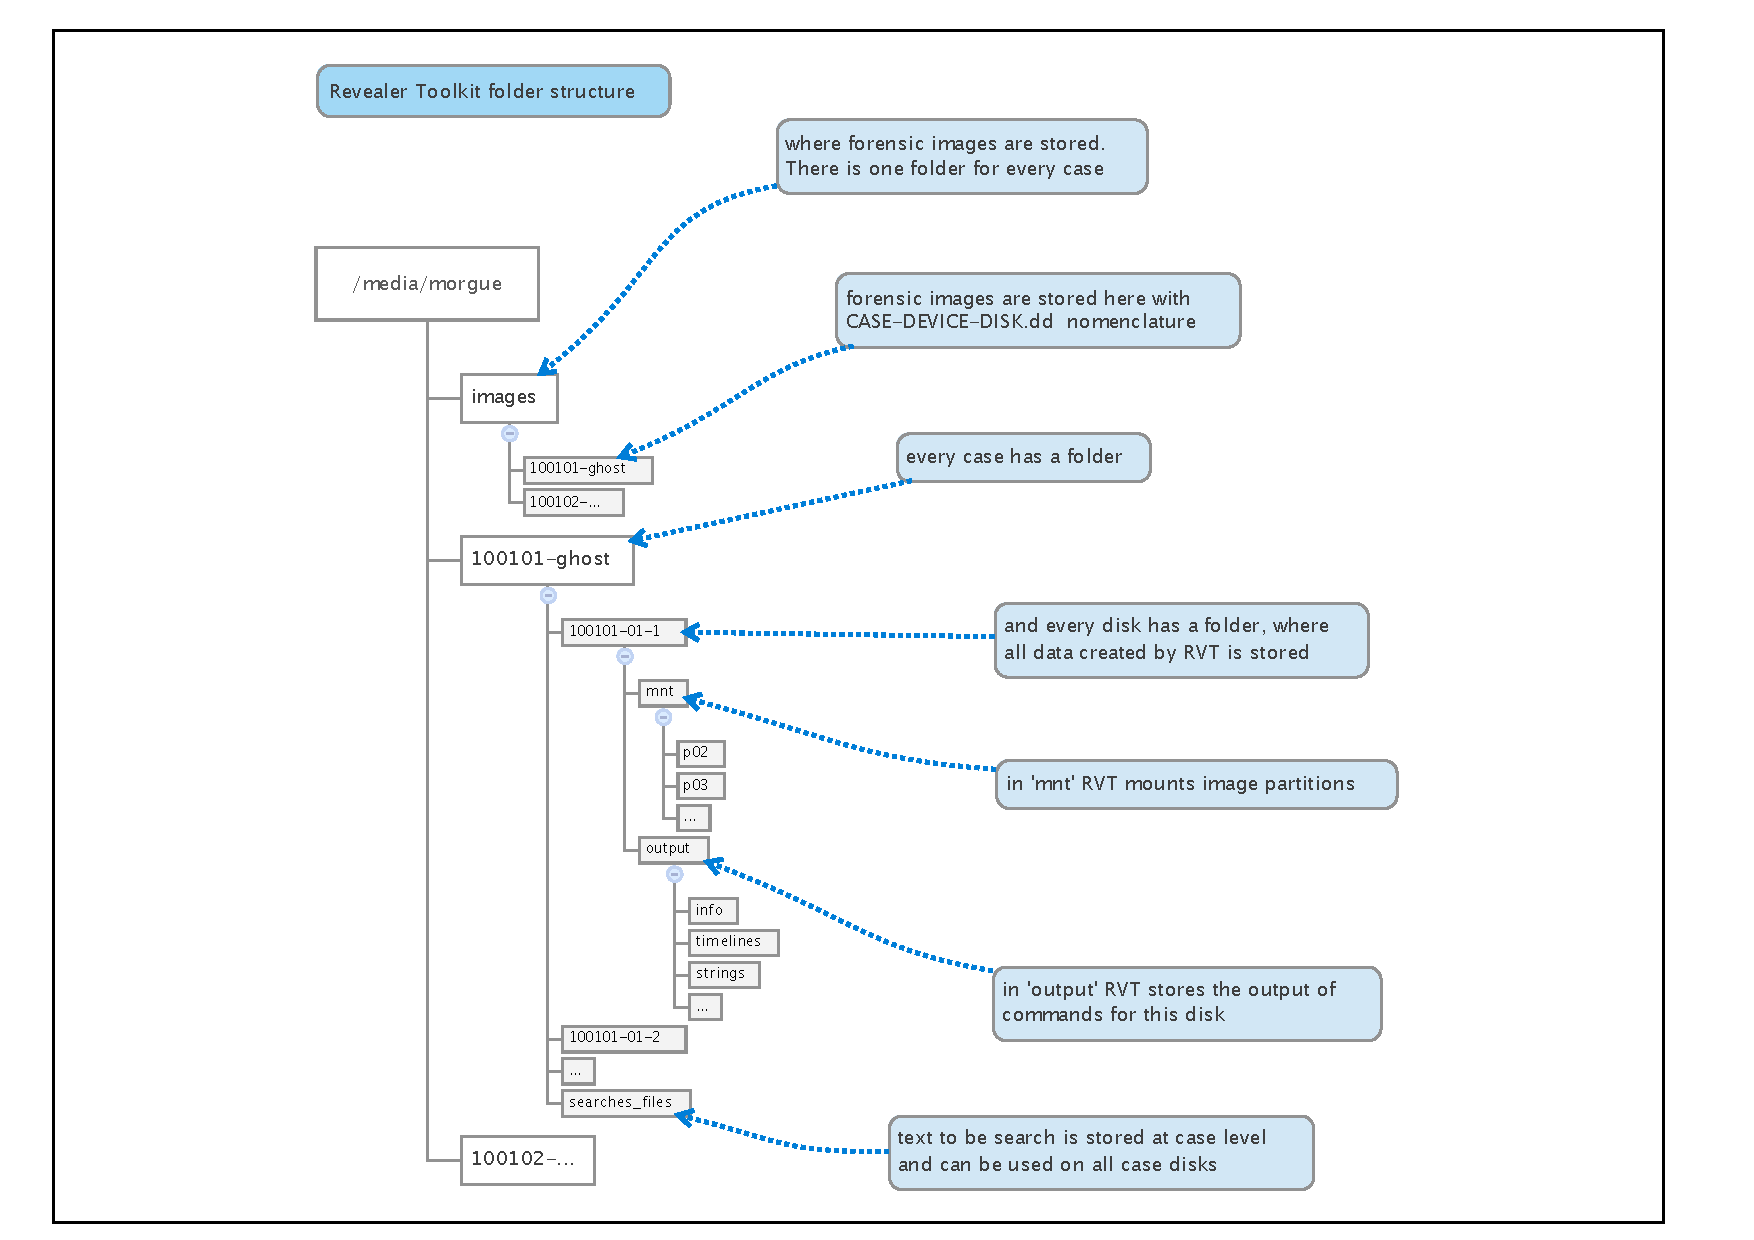
\includegraphics[width=\textheight,angle=270]{images/RVT_folder_structure.pdf} 
\caption{RVT folder structure} \label{img:folderstructure}
\end{figure}



\section{Morgues}

The Revealer Toolkit can handle more that one morgue. By default, one morgue is defined in RVT, located at \emph{/media/morgue}. 



\section{Cases}

Each forensic case is determined by a \emph{case number} and a \emph{case codename}, separated by a dash. For example, the example case created in the Chapter \ref{sec:installation} is noted as \emph{100101-ghost}.

Each case has a folder assigned in the morgue, under the folder \emph{images}, where the disk images are stored.

Also, each case has a folder in the morgue, where all the forensic results are stored.

The folder structure, at the case level, for the example installation shown in chapter \ref{sec:installation}, will be:

\begin{verbatim}
/media/morgue/100101-ghost

/media/morgue/imagenes/100101-ghost
/media/morgue/imagenes/100101-ghost/100101-01-1.dd
\end{verbatim}

where \emph{100101-01-1.dd} is the dd image of a disk.


\section{Devices, disks and partitions}

Under the Revealer Toolkit, information sources are organized with:

\begin{itemize}
\item Devices: each case has a number of devices: computers, cell phones, digital cameras, ...   They are numbered sequencially from 01 to 99. 

A device is named as \emph{casenumber-devicenumber}, for example, \emph{100101-01} for the case 100101 and device 01.

\item Disks: each device has a number of disks: hard disks, CD's, memory cards, ... They are numbered sequencially from 1 to 9

A disk is named as \emph{case-device-disknumber}, for example, \emph{100101-01-1}, for the disk 1

\item Partitions:  each disk can have several partitions, numbered from 01 to 99. The numeration used by the Sleuthkit command \emph{mmls} is used.

A partition is noted as \emph{case-device-disk-ppartition}, for example, 100101-01-1-p02 for partition 02.
\end{itemize}


Under each case folder, a folder must exist for every disk to be analyzed. 

This folder structure, at a disk level, for the example installation shown in chapter \ref{sec:installation}, will be:

\begin{verbatim}
/media/morgue/100101-ghost
/media/morgue/100101-ghost/100101-01-1

/media/morgue/imagenes/100101-ghost
/media/morgue/imagenes/100101-ghost/100101-01-1.dd
\end{verbatim}


\section{Forensic results}

The Revealer Toolkit Shell manages and executes \emph{script modules}, which performs forensic operations on the disk images and disk information. The results of these script modules are stored in the corresponding disk folder, under a folder named \emph{output}.

The folder structure and file content stored here depends on each script module. See chapter \ref{sec:modules} for further information.

Furthermore, under the disk folder other folder exists, named \emph{mnt}, that contains the mounting points for the image partitions. 

Then, the complete folder structure for the example shown in chapter \ref{sec:installation} will be:

\begin{verbatim}
/media/morgue/100101-ghost
/media/morgue/100101-ghost/100101-01-1
/media/morgue/100101-ghost/100101-01-1/mnt
/media/morgue/100101-ghost/100101-01-1/output

/media/morgue/imagenes/100101-ghost
/media/morgue/imagenes/100101-ghost/100101-01-1.dd
\end{verbatim}


% -----------------------------------
% Command guide
% -----------------------------------


\chapter{Command guide}

The Revealer Toolkit Shell provide several commands used to (a) manage your forensic images and (b) execute forensic operations over them.

RVT Shell is a Perl script that, when executed, performs a scan of the morgue and of all the images stored into it. After that, a prompt is shown and commands can be introduced.



\section{General interaction}

\begin{itemize}
\item to execute one command, type it at the prompt, add the corresponding arguments, and type RETURN. Some commands return information on the screen, some, write information at the \emph{output} folder of the corresponding disk at the morgue. Other, do both.

\item type one command followed by \emph{?} to obtain help about it

\item type the TAB key to obtain a list of available commands

\end{itemize}

\begin{verbatim}
Welcome to Revealer Tools Shell (v0.2):

 RVT  > 
        case
        cluster
        images
        info
        inode
        losetup
        mount
        script
        set
        test
 RVT  > 
\end{verbatim}





\section{Cheatsheets}

For those who know the name of the game, the following tables could be used as quick reference.

\begin{itemize}
\item Command quick reference, Table \ref{tbl:cmd-ref}, page \pageref{tbl:cmd-ref}
\item Script modules quick reference, Table \ref{tbl:scr-ref}, page \pageref{tbl:scr-ref}
\end{itemize}


\begin{table}[p]
\footnotesize


\begin{tabular}{| p{1cm}  p{10cm} | }

\hline 

\multicolumn{2}{|l|}{\it \bf
case list
} \\
 & lists cases in the morgue \\

\hline \hline

\multicolumn{2}{|l|}{\it \bf
images list
} \\
 & lists images in the morgue \\

\hline \hline

\multicolumn{2}{|l|}{\it \bf
images partition info $<$partition$>$
} \\
 & prints partition's information  \\

\multicolumn{2}{|l|}{\it \bf
images partition table $<$disk$>$
} \\
 &  prints partitions of a disk \\

\multicolumn{2}{|l|}{\it \bf
images loadconfig
} \\
 & Loads the morgue config from XML file \\

\hline \hline

\multicolumn{2}{|l|}{\it \bf
info list
} \\
 & shows some morgue's information \\

\multicolumn{2}{|l|}{\it \bf
info debug $<$dumpmorguexml$|$dumprvtcases$|$dumprvtcfg$>$
} \\
 & prints part of the RVT internal configuration  \\

\hline \hline


\multicolumn{2}{|l|}{\it \bf
losetup assign $<$disk$|$partition$>$
} \\
 & assigns a loop device to the partition \\

\multicolumn{2}{|l|}{\it \bf
losetup delete $<$disk$|$partition$>$
} \\
 & deletes a loop device assign to the partition \\

\multicolumn{2}{|l|}{\it \bf
losetup list 
} \\
 & lists the losetups devices assigned to RVT partitions \\

\multicolumn{2}{|l|}{\it \bf
losetup recheck
} \\
 & updates RVT internal configuration on loop devices \\

\hline \hline

\multicolumn{2}{|l|}{\it \bf
mount assign $<$disk$|$partition$>$
} \\
 & mounts a partition \\

\multicolumn{2}{|l|}{\it \bf
mount delete $<$disk$|$partition$>$
} \\
 & umounts a partition \\

\multicolumn{2}{|l|}{\it \bf
mount list 
} \\
 & list mounted RVT partitions \\

\multicolumn{2}{|l|}{\it \bf
mount recheck
} \\
 & updates RVT internal configuration on mounted partitions \\

\hline \hline

\multicolumn{2}{|l|}{\it \bf
cluster allocationstatus $<$cluster$>$ $<$partition$>$
} \\
 & prints cluster allocation status \\


\multicolumn{2}{|l|}{\it \bf
cluster extract $<$raw$|$ascii$>$ $<$cluster[,num]$>$ $<$partition$>$
} \\
 & extracts a cluster, or \emph{num} clusters, from partition \\


\multicolumn{2}{|l|}{\it \bf
cluster generateindex $<$disk$>$
} \\
 & creates files for a cluster-inode quick resolution \\


\multicolumn{2}{|l|}{\it \bf
cluster toinode $<$cluster$>$ $<$partition$>$
} \\
 & prints all inodes associated with a cluster \\

\hline \hline

\multicolumn{2}{|l|}{\it \bf
inode allocationstatus $<$inode$>$ $<$partition$>$
} \\
 & prints inode allocation status \\

\hline \hline

\multicolumn{2}{|l|}{\it \bf
set level [$<$case$|$device$|$disk$|$partition$>$]
} \\
 & sets working case level \\

\hline

\end{tabular}

\caption{Command quick reference}\label{tbl:cmd-ref}


\end{table}




\begin{table}[p]
\footnotesize


\begin{tabular}{| p{1cm}  p{10cm} | }


\hline 

\multicolumn{2}{|l|}{\it \bf
script filelist generate $<$disk$>$
} \\
 & generates lists of files for each partition \\

\hline \hline

\multicolumn{2}{|l|}{\it \bf
script files allocfiles $<$disk$>$
} \\
 & generates lists of allocated files for each partition \\

\hline \hline

\multicolumn{2}{|l|}{\it \bf
script search clusterlist $<$file$>$ $<$disk$>$
} \\
 & builds a list of clusters and file paths from a previous search \\

\multicolumn{2}{|l|}{\it \bf
script search clusters $<$file$>$ $<$disk$>$
} \\
 & extract clusters that match a previous search \\

\multicolumn{2}{|l|}{\it \bf
script search file $<$delete$|$edit$|$list$|$show$>$
} \\
 &  manages search files \\

\multicolumn{2}{|l|}{\it \bf
script search launch $<$file$>$ $<$disk$>$
} \\
 & launches a search \\

\multicolumn{2}{|l|}{\it \bf
script search quickcount $<$name:regexpr$>$ $<$disk$>$
} \\
 & counts the appearance of a regular expression. Predefined regexpr: \emph{emails, accounts, ips}. \\

\hline \hline

\multicolumn{2}{|l|}{\it \bf
script strings generate $<$disk$>$
} \\
 & generates strings for all partitions of a disk \\

\hline \hline

\multicolumn{2}{|l|}{\it \bf
script timelines generate $<$disk$>$
} \\
 & generates timelines for all partitions of a disk \\

\hline \hline

\multicolumn{2}{|l|}{\it \bf
script regripper listmodules
} \\
 & list available RegRipper modules \\

\multicolumn{2}{|l|}{\it \bf
script repripper execmodule $<$plugin$>$ $<$hivetype$>$ $<$partition$>$
} \\
 & executes one RegRipper module on the last modified hive of the type specified partition \\

\multicolumn{2}{|l|}{\it \bf
script regripper execallmodules $<$hivetype$>$ $<$partition$>$
} \\
 & executes all RegRipper modules on all hive files on the specified partition \\

\hline \hline

\multicolumn{2}{|l|}{\it \bf
script mail parsepsts $<$partition$>$
} \\
 & parse all PST files on partition \\

\hline 



\end{tabular}

\caption{Modules quick reference}\label{tbl:scr-ref}


\end{table}






\section{Command: \emph{case}}

Case management.

\subsection{\emph{case list}}

Gives a list of the cases stored in the morgue.

\begin{verbatim}
 RVT  > case list
Cases in the morgue: 
        100101 'ghost':
                100101-01-1

 \end{verbatim}



\section{Command: \emph{images}}

Image management.



\subsection{\emph{images list}}

Gives a list of the disk images stored in the morgue.

\begin{verbatim}
 RVT  > images list
Images in the morgue: 
        100101 'ghost':
                100101-01-1.dd

\end{verbatim}



\subsection{\emph{images partition info}}

Gives information about a partition.

\begin{verbatim}
 RVT  > images partition info 100101-01-1-p03                                 

Info for partition  - 100101-01-1-p03:

Filesystem:     FAT12
Cluster size:   2048
Sector size:    512
Offset:         0000010240 sectors ( 5242880 bytes )
\end{verbatim}

\subsection{\emph{images partition table}}

Gives the partition table of an image.

\begin{verbatim}
 RVT  > images partition table 100101-01-1

        03:     6 MB    Linux (0x83)
        02:     5 MB    Linux (0x83)
\end{verbatim}


\subsection{\emph{images scanall}}

RVT scans the morgue. No output given. 

Necessary when adding a new image to the morgue. You can check what RVT thinks that is in your morgue executing \emph{info debug dumpmorguexml} (see \ref{cmd:info-debug})


\subsection{\emph{images loadconfig}}

Loads the morgue config from XML file.


\section{Command: \emph{info}}

Manages RVT Shell configuration information.

\subsection{\emph{info list}}

Gives RVT Shell configuration information.

\begin{verbatim}
 RVT  > info list

        List of morgues:
                /media/morgue 
                /media/datos 


        List of morgues of images:
                /media/morgue/imagenes 
                /media/datos/imagenes 
\end{verbatim}



\subsection{\emph{info debug}} \label{cmd:info-debug}

dump the content of some system variables, like RVT configuration or morgue status:

\begin{itemize}
\item \emph{info debug dumpmorguexml}: dumps content of \emph{RVTmorgueInfo.xml} as imported by RVT
\item \emph{info debug dumprvtcases}: dumps content of internal variable \emph{RVT\_cases} (for developers only)
\item \emph{info debug dumprvtcfg}: dumps content of current RVT configuration
\end{itemize}

\begin{verbatim}
 RVT  > info debug dumprvtcfg                                                 

\$VAR1 = {
          'morgueInfoXML' => '/media/morgue/RVTmorgueInfo.xml',
          'log_level' => '0',
          'mount_gid' => '1010',
          'mount_umask' => '007',
          'paths' => [
                     {
                       'images' => [
                                   '/media/morgue/images'
                                 ],
                       'morgues' => [
                                    '/media/morgue'
                                  ],
                       'tmp' => '/tmp'
                     }
                   ],
          'tsk_path' => '/usr/local/bin'
        };
\end{verbatim}






\section{Command: \emph{losetup}}

Loop device management.

\subsection{\emph{losetup assign}}

Assigns a loop device to each partition of a case, disk or partition

\begin{verbatim}
 RVT  > losetup assign 100101

sudo losetup -f /media/morgue/imagenes/100101-ghost/100101-01-1.dd -o 5242880

sudo losetup -f /media/morgue/imagenes/100101-ghost/100101-01-1.dd -o 5120
\end{verbatim}


\subsection{\emph{losetup delete}}

Delete loop devices assigned to a case, disk or partition

\begin{verbatim}
 RVT  > losetup delete 100101
\end{verbatim}


\subsection{\emph{losetup list}}

List all loop devices assigned.

\begin{verbatim}
 RVT  > losetup list                                                          
Loop devices: 
        loop1   100101-01-1.dd  5120
        loop0   100101-01-1.dd  5242880
\end{verbatim}


\subsection{\emph{losetup recheck}}

Updates loop device information from the operating system.


\section{Command: \emph{mount}}

Mount points management.

\subsection{\emph{mount assign}}

Mounts the partitions of a case, disk or partition at the path \emph{morgue/100xxx-case/100xxx-device-disk/mnt/p0N}, where N is the partition number.

\begin{verbatim}
 RVT  > mount assign 100101

sudo mount /media/morgue/imagenes/100101-ghost/100101-01-1.dd /media/morgue/100101-ghost/100101-01-1/mnt/p03 -o ro,loop,iocharset=utf8,offset=5242880,umask=007,gid=1001

sudo mount /media/morgue/imagenes/100101-ghost/100101-01-1.dd /media/morgue/100101-ghost/100101-01-1/mnt/p02 -o ro,loop,iocharset=utf8,offset=5120,umask=007,gid=1001
\end{verbatim}


\subsection{\emph{mount delete}}

Umounts partitions of a case, disk or partition

\begin{verbatim}
 RVT  > mount delete 100101
\end{verbatim}


\subsection{\emph{mount list}}

List all mounted points.

\begin{verbatim}
 RVT  > mount list
Mounted partitions: 
        100101-01-1.dd  loop=/dev/loop0 offset=5242880
        100101-01-1.dd  loop=/dev/loop1 offset=5120
\end{verbatim}


\subsection{\emph{mount recheck}}

Updates mount points information from the operating system.



\section{Command: \emph{cluster}}

Operations on clusters.

\subsection{\emph{cluster allocationstatus}}

Prints cluster allocation status

\begin{verbatim}
 RVT  > cluster allocationstatus 2 100101-01-1-p02
Cluster 2: Allocated (Meta)
\end{verbatim}


\subsection{\emph{cluster extract}}

Prints the contents of the cluster. First argument specifies a post-treatment done to the cluster content before printing:

\begin{itemize}
\item raw:  prints original cluster without changes
\item ascii:  only prints ascii characters. Others are substituted with a dot
\end{itemize}

Second argument is the cluster number to be extracted. When the cluster number is appended with a comma and a integer number, extracts this number of consecutive clusters. For example, \emph{cluster extract raw 100,2 100101-01-1-p02} extracts clusters 100 and 101.

\begin{verbatim}
 RVT  > cluster extract ascii 3 100101-01-1-p02                                     
--------------------------------------------
/usr/bin/blkcat -o 0000000001 /media/morgue/imagenes/100101-espejismo/100101-01-1.dd 3 | 
\end{verbatim}


\subsection{\emph{cluster generateindex}}

Creates sort of an index for quick cluster-to-inode resolution. Required for performing searches. This is one of the few commands that writes files on the morgue.

See \emph{script search} (página \pageref{anx:searches} module for more information.


\subsection{\emph{cluster toinode}}

Prints all the inodes associated with a cluster.

\begin{verbatim}
 RVT  > cluster toinode 2 100101-01-1-p02                                     

inodes:

159700
\end{verbatim}



\section{Command: \emph{inode}}

Operations on inodes

\subsection{\emph{inode allocationstatus}}

Prints inode allocation status

\begin{verbatim}
 RVT  > inode allocationstatus 2 100101-01-1-p02

inode 2: Allocated
\end{verbatim}



\section{Command: \emph{script}}

Modular scripts. Each module is explained in a separated chapter (see Chapter \ref{sec:modules} for further information)


\section{Command: \emph{set}}

Sets RVT Shell configuration information.

\subsection{\emph{set level}}  \label{cmd:set-level}

Sets the work level to a specific case, device, disk or partition. When the work level is stablished, is notified at the prompt and there is no need of indicate it as argument at the commands.

\begin{verbatim}

 RVT  > images partition table 100101-01-1                                    

        03:     6 MB    Linux (0x83)
        02:     5 MB    Linux (0x83)

 RVT  > 
 RVT  > images partition table


I don't know what is this

 RVT  > set level 100101-01-1                                                 

 new format: disk
 RVT 100101-01-1 > images partition table                                     

        03:     6 MB    Linux (0x83)
        02:     5 MB    Linux (0x83)

 RVT 100101-01-1 > 
\end{verbatim}












\chapter{Script modules} \label{sec:modules}

Scripts modules are forensic software components that perform specific forensic tasks on the stored images and information.

Each module has particular objectives, methods, arguments and results, the documentation of which is detailed in the following sections.





\section{\emph{script filelist}}

Module for automatic generation of file lists in every partition. Mainly oriented to Windows filesystems, does not show permissions, owner, or group.

\subsection{\emph{script filelist generate}} 

Generates file lists for all partitions of a disk

\begin{verbatim}
script filelist generate <disk>
\end{verbatim}

It creates several files in the morgue with this path and name:

\begin{verbatim}
output/FileList/<disk>-p<partition>_FileList.csv
\end{verbatim}






\section{\emph{script files}}

Module for performing operations on mounted images.

\subsection{\emph{script files allocfiles}} 

Creates a file with a list of all the allocated files of the image.

\begin{verbatim}
files allocfiles <disk>
\end{verbatim}

It creates a file in the morgue with this path and name:

\begin{verbatim}
<morguepath>/<case>/<disk>/output/info/alloc_files.txt
\end{verbatim}

with a list of allocated files and folders.





\section{\emph{script search}} \label{anx:searches}

Module for performing searches. See the Appendix \ref{anx:searches} for a step-by-step tutorial.


\subsection{\emph{script search clusterlist}}

Builds a list of clusters and file paths that matches a previous search.

\begin{verbatim}
script search clusterlist <search file> <image>
\end{verbatim}

It creates several files in the morgue with this path and name:

\begin{verbatim}
<morguepath>/<case>/<disk>/output/searches/cbusq_<search>-<partition>
<morguepath>/<case>/<disk>/output/searches/pbusq_<search>-<partition>
\end{verbatim}

with this format:

cbusq:
\begin{verbatim}
<cluster>:<inode>:<allocation status>:<file path>
\end{verbatim}

pbusq:
\begin{verbatim}
<file path> (<allocation status)
\end{verbatim}



\subsection{\emph{script search clusters}}

Extract the clusters matched in a previous search

\begin{verbatim}
script search clusters <search file> <image>
\end{verbatim}

It creates several files in the morgue with this path and name:

\begin{verbatim}
<morguepath>/<case>/<disk>/output/searches/ibusq_<search>-<partition>
\end{verbatim}

with this format:

\begin{verbatim}
---------------------------
<byte offset>:<cluster>:<allocation status>:  <line that matches search>

<cluster content>
\end{verbatim}


\subsection{\emph{script search file}}

Commands to manage search files:

\begin{itemize}
\item	script search file delete $<$name$>$:  deletes file
\item	script search file edit $<$name$>$:  creates and/or edit file with \emph{vim}
\item	script search file list:  lists search files created
\item	script search file show $<$name$>$:  prints file's contents
\end{itemize}

The files are created per case, and are stored at this path:

\begin{verbatim}
<morguepath>/<case>/searches_files
\end{verbatim}


\subsection{\emph{script search launch}}

Launches a search in an image. 

\begin{verbatim}
script search launch <search file> <image>
\end{verbatim}

It creates several files in the morgue with this path and name:

\begin{verbatim}
<morguepath>/<case>/<disk>/output/searches/busq_<search>
\end{verbatim}

with this format:

\begin{verbatim}
<strings file that matches>: <byte offset> <line that matches>
\end{verbatim}



\subsection{\emph{script search quickcount}}

Launch a quick search in a case or in an image with a count of the results.

\begin{verbatim}
script search quickcount <name:regular expression>  <image>
\end{verbatim}

It creates several files in the morgue with this path and name:

\begin{verbatim}
<morguepath>/<case>/<disk>/output/info/count_<name>
\end{verbatim}

with this format:

\begin{verbatim}
<times that the match appear>  <match>
\end{verbatim}

There are some quickcounts preconfigured:

\begin{itemize}
\item script search quickcount emails $<$image$>$: search emails addresses
\item script search quickcount accounts $<$image$>$: search bank accounts
\item script search quickcount ips $<$image$>$: search ip addresses
\item script search quickcount phones $<$image$>$: search phone numbers
\end{itemize}




\section{\emph{script strings}}

Module for creating and managing string files of images.

\subsection{\emph{script strings generate}} 

Generates strings for all partitions of a disk 

\begin{verbatim}
script strings generate <disk>
\end{verbatim}

It creates several files in the morgue with this path and name:

\begin{verbatim}
<morguepath>/<case>/<disk>/output/strings/strings-<case>-<partition>.asc
<morguepath>/<case>/<disk>/output/strings/strings-<case>-<partition>.uni
\end{verbatim}

Strings files of ASCII characters have \emph{.asc} extension.

Strings files of Unicode (UTF8) characters have \emph{.uni} extension.





\section{\emph{script timelines}}

Module for creating and managing timelines.

\subsection{\emph{script timelines generate}} 

Generates timelines for all partitions of a disk

\begin{verbatim}
script timelines generate <disk>
\end{verbatim}

It creates several files in the morgue with this path and name:

\begin{verbatim}
output/timelines/<disk>-p<partition>_iTL.csv
output/timelines/<disk>-p<partition>_iTL-day.sum
output/timelines/<disk>_TL.csv
output/timelines/<disk>_TL.txt
output/timelines/<disk>_TL-day.sum
output/timelines/<disk>_TL-hour.sum
\end{verbatim}

Where \emph{i}timelines (from now on \textbf{iTL}) are calculated based on inodes, and timelines, with file names. \emph{day} and \emph{hour} sums are line counts grouped by days and hours.




\section{\emph{script webmail}}

Module for detecting and managing webmail.

Deprecated. Has to be rewritten.


\section{\emph{script software}}

Module for detecting software.

Deprecated. Has to be rewritten.


\section{\emph{script regripper}}

Module for parsing Microsoft Windows registry hives using RegRipper (www.regripper.net). See section \ref{anx:regripper} for notes about its installation.

\subsection{\emph{script regripper listmodules}}

List all RegRipper available modules. If this command does not return anything, please refer to section \ref{anx:regripper} for notes about RegRipper installation.



\subsection{\emph{script regripper execmodule}}

Executes one RegRipper module of a particular hive type on a partition. RVT picks the most suitable hive file (simply, it gets the most recent modified hive), and prints results on the screen.

\begin{verbatim}
script regripper execmodule <plugin> <hivetype> <partition>
\end{verbatim}

where $<$hivetype$>$ can be one of these: sam, security, software, system or ntuser



\subsection{\emph{script regripper execallmodules}}

Execute all RegRipper modules on all the hive files on a partition.

\begin{verbatim}
script regripper execallmodules  <hivetype> <partition>
\end{verbatim}

where $<$hivetype$>$ can be one of these: sam, security, software, system, ntuser  \textbf{or} all 

It stores the results on this folder \emph{output/regripper}, one file result per hive file, with this format:

\begin{verbatim}
output/regripper/<hivetype>-<last modified data>
\end{verbatim}

The first line of each results file have the path to the hive file on which RegRipper has been executed. 





\section{\emph{script mail}}

Module for extract emails in text format from Microsoft Outlook mailboxes (PST) using \emph{libpst} (www.five-ten-sg.com/libpst).

\subsection{\emph{script mail parsepsts}}

Search all Microsoft Outlook mailboxes (PST extension) and parse them with \emph{libpst}

\begin{verbatim}
script mail parsepsts <partition>
\end{verbatim}

Results are stored under \emph{output/mail}, where a folder is created for each PST file with the format:

\begin{verbatim}
output/mail/pst-n
\end{verbatim}

where \emph{n} is a increasing integer number.



\chapter{Operational guides and tricks}



\section{RVT Shell tricks}

The Revealer Toolkit can accept commands by several ways. One of them is through a shell. This section will provide you with some tricks to ease your interaction with RVT.

Yes, you will feel that RVT Shell is buggy and that lacks support for some keys, terminals and functionality, but, well, I made it myself and it is not perfect. It will be improved or substituted in future versions. Suggestions are welcome.


\subsection{command level}

Commands in RVT are \emph{nested} in levels. Each command level can contain commands, but also other command levels. You can enter a level entering its name in RVT Shell, and the RVT prompt will be modified.

For example, in order to execute the following commands, they can be written directly to RVT ...

\begin{verbatim}
RVT > info list
...
RVT > info debug dumpmorguexml
...
RVT > info debug dumprvtcases
...
RVT > info debug dumprvtcfg
...
\end{verbatim}


... but the following session, taking profit of command levels, also is possible:

\begin{verbatim}
 RVT  > info 
 RVT  info> list
 ...  
 RVT  info> debug
 RVT  info debug> dumpmorguexml
 ...
 RVT  info debug> dumprvtcases
 ...
 RVT  info debug> dumprvtcfg
 ...
\end{verbatim}


To go up one level, enter `\emph{r}':

\begin{verbatim}
RVT  info debug> r
RVT  info> r
RVT  > 
\end{verbatim}


\subsection{case level}

When working with a case or disk, usually you will have to type a lot of types this case or disk number because a lot of commands need it as argument. The \emph{set level} command (see section \ref{cmd:set-level}) will ease you user experience because it fixes a `case level' for the session. Commands that expect a case, device, disk or partition as an argument will use the `case level' established by \emph{set level} when the argument is not provided. 

The case level can be changed with other \emph{set level} command, and erased when executing \emph{set level} without arguments.

For example:

\begin{verbatim}

 RVT  > images partition table 100101-01-1                                    

        03:     6 MB    Linux (0x83)
        02:     5 MB    Linux (0x83)

 RVT  > 
 RVT  > images partition table


I don't know what is this

 RVT  > set level 100101-01-1                                                 

 new format: disk
 RVT 100101-01-1 > images partition table                                     

        03:     6 MB    Linux (0x83)
        02:     5 MB    Linux (0x83)

 RVT 100101-01-1 > 
\end{verbatim}


Moreover, case level can be determined as an argument to RVT itself:

\begin{verbatim}
$ rvt -l 100101-01-1
Scanning morgues. Please wait ...



Welcome to Revealer Tools Shell (v0.2):


 new format: disk
 RVT 100101-01-1 >  
\end{verbatim}



\subsection{TAB key}

When using the RVT Shell, the TAB key can be used in two ways:

\begin{enumerate}
\item at a command level, before writing, will show the available commands and levels
\item when a command or level is half written, will show the available command and levels that begin with the fragment that is written
\end{enumerate}

For example:

\begin{verbatim}
 RVT  >  <TAB>	
	case
	cluster
	images
	info
	inode
	losetup
	mount
	script
	set
	test
 RVT  > i<TAB>	
	images
	info
	inode
 RVT  > in<TAB>	
	info
	inode
\end{verbatim}


\subsection{command history}

RVT Shell provide a very simple history feature, which consist of remembering the last command typed, that can be accessed type the up arrow.

Future versions will improve the command history with bigger \emph{memory}.






\section{entities expansion}

Several commands recive a entity as an argument (a case, a device, a disk or a partition).  In some cases, is useful that a command could be applied to all the subentities below a entity of higher level. This could be achieved with \emph{entities expansion}.

For example, the command 

\begin{verbatim}
mount assign 100101-01-1-p02
\end{verbatim}

 will mount the 02 partition of the disk \emph{100101-01-1}.  But, what if 100101-01-1 have six partitions? and what if 100101 case have ten disks, every one of them with six partitions?

RVT will apply, automaticaly, a command to a group of subentities below a entity of higher level when the operands '@devices', '@disks' or '@partitions' are used just after the entity argument.

For example, the following command will mount all partitions of all disks of all devices of a case:

\begin{verbatim}
mount assign 100101@partitions
\end{verbatim}

Other example: the following command will launch a search on all de disks of a case:

\begin{verbatim}
script search launch mysearches 100101@disks
\end{verbatim}


\textbf{Note:} you will see that \emph{mount assign 100101}, without entity expansion, also mounts all partitions of the case 100101. The reason is that some commands, coded before entity expansion, have internal support for managing several types of entites


\section{chaining commands}

Some of the RVT commands can take a long time to execute. If want to execute a list of commands sequencially you can choose between two options.

On one hand, RVT Shell will execute sequencially commands separated by ';'. One example:

\begin{verbatim}
 RVT  > case list; images list

Cases in the morgue: 
	100101 'espejismo':
		100101-03-1
		100101-02-1


Images in the morgue: 
	100101 'espejismo':
		100101-01-2.dd
		100101-01-1.dd
		100101-03-1.dd
		100101-02-1.dd
\end{verbatim}

On the other hand, you can create a file containing a command on each line, and pipe them to RVT in batch mode (-b argument). For example:

\begin{verbatim}
$ cat commands.rvt 
case list
images list
$
$ cat commands.rvt | rvt -b

Welcome to Revealer Tools Shell (v0.2):

 RVT  > case list

Cases in the morgue: 
	100101 'espejismo':
		100101-03-1
		100101-02-1

images list

Images in the morgue: 
	100101 'espejismo':
		100101-01-2.dd
		100101-01-1.dd
		100101-03-1.dd
		100101-02-1.dd

$
\end{verbatim}


and, of course:


\begin{verbatim}
 
$ echo "case list; images list" |  rvt -b

Welcome to Revealer Tools Shell (v0.2):

 RVT  > case list

Cases in the morgue: 
	100101 'espejismo':
		100101-03-1
		100101-02-1

images list

Images in the morgue: 
	100101 'espejismo':
		100101-01-2.dd
		100101-01-1.dd
		100101-03-1.dd
		100101-02-1.dd

$
\end{verbatim}





\section{Logs}

RVT will log its activity to the local syslog, including commands launched, time and date, error messages, IP from the user (in the case that access to the RVT server is done with ssh), and a bit more.

For example, this unix command will show you the last RVT log messages:

{ \footnotesize
\begin{verbatim}
# grep 'RVT: ' /var/log/syslog
Jun 12 19:31:42 revealer RVT: INFO root@192.168.1.10 executing : RVT_images_list  
Jun 12 19:31:42 revealer RVT: INFO root@192.168.1.10 ending session 
Jun 12 19:31:53 revealer RVT: INFO root@192.168.1.10 starting up RVT v0.2 
Jun 12 19:31:53 revealer RVT: INFO root@192.168.1.10 loading configuration 
Jun 12 19:31:53 revealer RVT: INFO root@192.168.1.10 Morgue XML configuration loaded. Last updated: 2009061216:17:42 
Jun 12 19:31:53 revealer RVT: INFO root@192.168.1.10 Run 'images scanall' command to update 
Jun 12 19:31:53 revealer RVT: INFO root@192.168.1.10 RVT shell started 
Jun 12 19:31:53 revealer RVT: INFO root@192.168.1.10 executing : RVT_case_list  
Jun 12 19:31:53 revealer RVT: INFO root@192.168.1.10 executing : RVT_images_list  
Jun 12 19:31:53 revealer RVT: INFO root@192.168.1.10 ending session 

...
\end{verbatim}
}

and this, the commands on a particular disk:

{ \footnotesize
\begin{verbatim}
# grep '100101-03-1' syslog | grep 'executing'

Jun 12 16:17:56 revealer RVT: INFO root@192.168.1.10 executing : RVT_images_partition_table 100101-03-1 
Jun 12 16:18:37 revealer RVT: INFO root@192.168.1.10 executing : RVT_set_level 100101-03-1 
Jun 12 16:18:43 revealer RVT: INFO root@192.168.1.10 executing 100101-03-1: RVT_script_timelines_generate  
Jun 12 16:19:06 revealer RVT: INFO root@192.168.1.10 executing : RVT_set_level 100101-03-1 
Jun 12 16:19:11 revealer RVT: INFO root@192.168.1.10 executing 100101-03-1: RVT_script_timelines_generate  
Jun 12 16:19:27 revealer RVT: INFO root@192.168.1.10 executing 100101-03-1: RVT_mount_assign  
Jun 12 16:19:36 revealer RVT: INFO root@192.168.1.10 executing 100101-03-1: RVT_script_files_allocfiles  
Jun 12 18:34:18 revealer RVT: INFO root@192.168.1.10 executing : RVT_inode_allocationstatus 2 100101-03-1-p02 
Jun 12 18:34:44 revealer RVT: INFO root@192.168.1.10 executing : RVT_inode_allocationstatus 2 100101-03-1-p02 
Jun 12 18:53:38 revealer RVT: INFO root@192.168.1.10 executing : RVT_mount_delete 100101-03-1-p02

...
\end{verbatim}
}



\section{Searches} \label{anx:searches}

The Revealer Toolkit can perform searches on forensic images. Several commands are required to be executed to perform a search, that are discussed in this section.

The following two commands commands are required to be executed once before launching searches on a disk:

\begin{itemize}
\item \emph{script strings generate $<$disk$>$}:  extracts ascii and unicode strings from forensic image 
\item \emph{cluster generateindex $<$disk$>$}:  create a index for quick cluster--inode resolution
\end{itemize}

Next step is to create a file that contains the terms to be searched. These files can be created with RVT commands, and are visible to all disks on a case:

\begin{itemize}
\item \emph{script file edit $<$file name$>$}: this command opens a \emph{vim} file editor, that can be used to write a search term on each line. Writing the file and exiting \emph{vim} returns to RVT and a file is created in the directory $<$case$>$/searches\_files 
\end{itemize}

\textbf{Warning!:}  these rules apply when creating search terms (sorry, these limitations will be eliminated in future versions):

\begin{enumerate}
\item search is always case insensitive. Also, always write search terms in lower case
\item do not include characters outside ASCII charset (no accents, no ñ's, ...) So, for example, you cannot search "barça campió", so you have to search "a campi" instead. 
\item some regular expression characters can be used, although escape sequences have not been well tested. So, you can use '.', '*', '?', but not backslash or complex regular expressions 
\end{enumerate}

Now, searches can be launched. Three commands create different output related with a search file:

\begin{itemize}
\item \emph{script search launch $<$file name$>$}:   greps every search term on $<$file name$>$ over the strings files. Results are stored on \emph{output/searches/busq\_ $<$search term$>$}
\item \emph{script search clusters $<$file name$>$}:    for each \emph{busq\_} file generated before, extract the cluster that contains the term searched and writes the results on \emph{output/searches/ibusq\_$<$search term$>$}
\item \emph{script search clusterlist $<$file name$>$}:   it takes each \emph{busq\_} file generated before and creates two new files: \emph{cbusq\_$<$search term$>$}, which contains a list of clusters that contain the searched terms, its allocation status and path if allocated, and  \emph{pbusq\_$<$search term$>$}, which contains a list of paths associated with allocated clusters that contains search terms\footnote{beware! if search terms are allocated on slack space, files could be included in the pbusq file that do actually not include this search term (because is on the slack space!)}
\end{itemize}

Now, you are ready to review megabytes and megabytes of results, that are stored under disk folder \emph{output/searches}, in a black shell window   :)

A typical search session could be like this, where the objective is to search the words `revealer' and `toolkit' on all disks of the case `100101-ghost':

\begin{verbatim}
RVT > set level 100101
RVT > script strings generate @disks
RVT > cluster generateindex @disks
RVT 100101 > script search
RVT 100101 script search > file edit myFile

(`i' key pressed on vim)
revealer
toolkit
(ESC key pressed and then `:wq' to write and exit back to RVT)

RVT 100101 script search > launch myFile @disks; clusters myFile @disks; 
 clusterlist myFile @disks

\end{verbatim}





\section{F-Response compatibility}

The Revealer Toolkit is fully compatible with F-Reponse (www.f-response.com), that is, forensic tasks on remote F-Response disks can be automated through RVT. 

\emph{But}, RVT is \emph{optimized} to be used with F-Response, so expect a considerable load of time and network traffic on some operations.

In order to use a F-Response created device, or, in general, any disk device as a RVT image, create a symbolic link to it from the \emph{images} directory (f.ex., \emph{ln -s /dev/sdx /media/morgue/images/ 100101-ghost/100101-02-1.dd})

Future versions will include RVT commands for managing F-Response targets and devices.




\section{Known problems}

Remember that RVT is not stable yet, so there are some problems pending to be solved in future versions:


\begin{itemize}

\item error verbosity:  RVT do not offer a lot of verbosity when an error occurs

\item commands dependences:  to be executed, each command has a list of dependences: executables installed on the system, other commands have to be executed before, arguments, ...  Sometimes, a command fails because one dependence is not found and is not checked automatically before executing

\item keyboard does not work as expected:  RVT Shell code is very simple, and it does not handle properly a lot of keyboard actions, as movement arrows, delete keys, etc. This problem is worse when working with remote terminals, screens, and other shell tricks

\item search engine has to be improved

\item ... 

\end{itemize}




\appendix




\chapter{Sample image from scratch} \label{anx:scratch}

Sometimes could be useful to create an image from scratch. A simple procedure is provided in order to create such image from linux.

as user:

\begin{verbatim}
cd /media/morgue/imagenes/100101-ghost/
dd if=/dev/zero bs=1024 count=10240 > 100101-01-1.dd
\end{verbatim}

as root:

\begin{verbatim}
fdisk /media/morgue/imagenes/100101-ghost/100101-01-1.dd

in fdisk:

x (additional functions)

c (cylinders)
1024
s (sectors)
10
h (heads)
2

r (main menu)
n (new partition)
p 
1
1   (first cylinder)
512 (half of the disk)
n (new partition)
p 
2
513 (half of the disk)
1024 (last cylinder)
w (save and exit)
\end{verbatim}

and now, let's put some info inside, as root:

\begin{verbatim}
echo "images scanall; losetup assign 100101-01-1; losetup list" | RVT.pl -b
   (the last command reveals loop devices created)
mkfs.vfat /dev/loop0
mkfs.vfat -F 32 /dev/loop1   

mkdir /media/aux1
mount /dev/loop0 /media/aux1
cp /home/analyst/RVT/RVT.pl /media/aux1
umount /media/aux1
mount /dev/loop1 /media/aux1
cp /home/analyst/RVT/RVT.pl /media/aux1
sync
rm /media/aux1/RVT.pl
echo "my email address is myemail@revealertoolkit.com" > /media/aux1/textfile.txt
umount /media/aux1

echo "losetup delete 100101-01-1" | RVT.pl -b
\end{verbatim}




\chapter{Additional software installation}


\section{libpst Utilities} \label{anx:libpst}

Download lastest stable package from http://www.five-ten-sg.com/libpst/packages, unzip and compile. After that, copy or link \emph{readpst} executable to \emph{/usr/local/bin}.

\begin{verbatim}
cd /usr/local/src
mkdir libpst
cd libpst
wget http://www.five-ten-sg.com/libpst/packages/libpst-0.6.37.tar.gz
tar -zxf libpst-0.6.37.tar.gz
cd libpst-0.6.37
./configure
make
cp src/readpst /usr/local/bin
\end{verbatim}



\section{RegRipper} \label{anx:regripper}

Download lastest stable package from www.regripper.net and unzip:

\begin{verbatim}
cpan Parse::Win32Registry

mkdir /usr/local/src/regripper
cd /usr/local/src/regripper
wget http://www.regripper.net/RegRipper/RegRipper/rr_20080909.zip
unzip rr_20080909.zip

apt-get install tofrodos
dos2unix rip.pl
\end{verbatim}


some changes have to be made on RegRipper code to be executable on Linux:

\begin{verbatim}
1c1
< #! c:\perl\bin\perl.exe
---
> #!/usr/bin/perl
29c29
< my $plugindir = "plugins\\";
---
> my $plugindir = "/usr/local/src/regripper/plugins/";
92c92
< 			require "plugins\\".$plugins{$i}."\.pl";
---
> 			require $plugindir.$plugins{$i}."\.pl";
\end{verbatim}

and final touches:

\begin{verbatim}
perl rip.pl -l > plugins/plugins

ln -s /usr/local/src/regripper/rip.pl /usr/local/bin/rip
chmod a+x /usr/local/src/regripper/rip.pl
\end{verbatim}


\end{document}